\documentclass{article}\usepackage[]{graphicx}\usepackage[]{color}
%% maxwidth is the original width if it is less than linewidth
%% otherwise use linewidth (to make sure the graphics do not exceed the margin)
\makeatletter
\def\maxwidth{ %
  \ifdim\Gin@nat@width>\linewidth
    \linewidth
  \else
    \Gin@nat@width
  \fi
}
\makeatother

\definecolor{fgcolor}{rgb}{0.345, 0.345, 0.345}
\newcommand{\hlnum}[1]{\textcolor[rgb]{0.686,0.059,0.569}{#1}}%
\newcommand{\hlstr}[1]{\textcolor[rgb]{0.192,0.494,0.8}{#1}}%
\newcommand{\hlcom}[1]{\textcolor[rgb]{0.678,0.584,0.686}{\textit{#1}}}%
\newcommand{\hlopt}[1]{\textcolor[rgb]{0,0,0}{#1}}%
\newcommand{\hlstd}[1]{\textcolor[rgb]{0.345,0.345,0.345}{#1}}%
\newcommand{\hlkwa}[1]{\textcolor[rgb]{0.161,0.373,0.58}{\textbf{#1}}}%
\newcommand{\hlkwb}[1]{\textcolor[rgb]{0.69,0.353,0.396}{#1}}%
\newcommand{\hlkwc}[1]{\textcolor[rgb]{0.333,0.667,0.333}{#1}}%
\newcommand{\hlkwd}[1]{\textcolor[rgb]{0.737,0.353,0.396}{\textbf{#1}}}%

\usepackage{framed}
\makeatletter
\newenvironment{kframe}{%
 \def\at@end@of@kframe{}%
 \ifinner\ifhmode%
  \def\at@end@of@kframe{\end{minipage}}%
  \begin{minipage}{\columnwidth}%
 \fi\fi%
 \def\FrameCommand##1{\hskip\@totalleftmargin \hskip-\fboxsep
 \colorbox{shadecolor}{##1}\hskip-\fboxsep
     % There is no \\@totalrightmargin, so:
     \hskip-\linewidth \hskip-\@totalleftmargin \hskip\columnwidth}%
 \MakeFramed {\advance\hsize-\width
   \@totalleftmargin\z@ \linewidth\hsize
   \@setminipage}}%
 {\par\unskip\endMakeFramed%
 \at@end@of@kframe}
\makeatother

\definecolor{shadecolor}{rgb}{.97, .97, .97}
\definecolor{messagecolor}{rgb}{0, 0, 0}
\definecolor{warningcolor}{rgb}{1, 0, 1}
\definecolor{errorcolor}{rgb}{1, 0, 0}
\newenvironment{knitrout}{}{} % an empty environment to be redefined in TeX

\usepackage{alltt}
\usepackage{geometry}
\usepackage{amsmath}
\usepackage{lscape}
\geometry{verbose,tmargin=2.5cm,bmargin=2.5cm,lmargin=2.5cm,rmargin=2.5cm}
\IfFileExists{upquote.sty}{\usepackage{upquote}}{}
\begin{document}




\title{Messina Experiment 1: Classical Survival Approaches}
\maketitle


%%%%%%%%%%%%%%%%%%%%%%%%%%%%%%%%%%%%%%%%%%%%%%%%%%%%%%%%%%%%%%%%%%%%%%
% LIBRARIES
%%%%%%%%%%%%%%%%%%%%%%%%%%%%%%%%%%%%%%%%%%%%%%%%%%%%%%%%%%%%%%%%%%%%%%
\section{Preparation}
\begin{knitrout}
\definecolor{shadecolor}{rgb}{0.969, 0.969, 0.969}\color{fgcolor}\begin{kframe}
\begin{alltt}
\hlkwd{library}\hlstd{(messina)}
\end{alltt}


{\ttfamily\noindent\itshape\color{messagecolor}{\#\# Loading required package: survival\\\#\# Loading required package: splines\\\#\# Loading required package: methods}}\begin{alltt}
\hlkwd{library}\hlstd{(plyr)}
\hlkwd{library}\hlstd{(reshape2)}
\hlkwd{library}\hlstd{(ggplot2)}

\hlkwd{library}\hlstd{(doMC)}
\end{alltt}


{\ttfamily\noindent\itshape\color{messagecolor}{\#\# Loading required package: foreach\\\#\# Loading required package: iterators\\\#\# Loading required package: parallel}}\begin{alltt}
\hlkwd{registerDoMC}\hlstd{(}\hlnum{32}\hlstd{)}
\end{alltt}
\end{kframe}
\end{knitrout}


%%%%%%%%%%%%%%%%%%%%%%%%%%%%%%%%%%%%%%%%%%%%%%%%%%%%%%%%%%%%%%%%%%%%%%
% FUNCTIONS
%%%%%%%%%%%%%%%%%%%%%%%%%%%%%%%%%%%%%%%%%%%%%%%%%%%%%%%%%%%%%%%%%%%%%%
\section{Accessory Functions}
\begin{knitrout}
\definecolor{shadecolor}{rgb}{0.969, 0.969, 0.969}\color{fgcolor}\begin{kframe}
\begin{alltt}
\hlstd{calcCensorWeibullRate} \hlkwb{=} \hlkwa{function}\hlstd{(}\hlkwc{surv.shape}\hlstd{,} \hlkwc{surv.scale}\hlstd{,} \hlkwc{cens.shape}\hlstd{,} \hlkwc{cens.scale}\hlstd{,} \hlkwc{plot} \hlstd{=} \hlnum{FALSE}\hlstd{)}
\hlstd{\{}
        \hlkwa{if} \hlstd{(plot)}
        \hlstd{\{}
                \hlstd{x} \hlkwb{=} \hlkwd{seq}\hlstd{(}\hlnum{0}\hlstd{,} \hlnum{10}\hlopt{*}\hlkwd{min}\hlstd{(surv.scale, cens.scale),} \hlkwc{length.out} \hlstd{=} \hlnum{1e4}\hlstd{)}
                \hlstd{y} \hlkwb{=} \hlkwd{dweibull}\hlstd{(x,} \hlkwc{shape} \hlstd{= cens.shape,} \hlkwc{scale} \hlstd{= cens.scale)} \hlopt{*} \hlstd{(}\hlnum{1} \hlopt{-} \hlkwd{pweibull}\hlstd{(x,} \hlkwc{shape} \hlstd{= surv.shape,} \hlkwc{scale} \hlstd{= surv.scale))}
                \hlkwd{plot}\hlstd{(y} \hlopt{~} \hlstd{x,} \hlkwc{type} \hlstd{=} \hlstr{"l"}\hlstd{)}
        \hlstd{\}}
        \hlkwd{integrate}\hlstd{(}\hlkwa{function}\hlstd{(}\hlkwc{t}\hlstd{)} \hlkwd{dweibull}\hlstd{(t,} \hlkwc{shape} \hlstd{= cens.shape,} \hlkwc{scale} \hlstd{= cens.scale)} \hlopt{*} \hlstd{(}\hlnum{1} \hlopt{-} \hlkwd{pweibull}\hlstd{(t,} \hlkwc{shape} \hlstd{= surv.shape,} \hlkwc{scale} \hlstd{= surv.scale)),} \hlkwc{lower} \hlstd{=} \hlnum{0.001}\hlstd{,} \hlkwc{upper} \hlstd{=} \hlnum{10}\hlopt{*}\hlkwd{min}\hlstd{(surv.scale, cens.scale))}\hlopt{$}\hlstd{value}
\hlstd{\}}
\hlcom{# calcCensorWeibullRate(1/0.7253, exp(6.9), 1/0.3216, exp(7.1))}
\hlcom{# temp.ws = rweibull(1e6, 1/0.7253, exp(6.9))}
\hlcom{# temp.wc = rweibull(1e6, 1/0.3216, exp(7.1))}
\hlcom{# mean(temp.wc < temp.ws)}
\hlcom{# AW FUK YEH}
\hlcom{# calcCensorWeibullRate(1.379,601.8,3.109,10188,plot = TRUE)}

\hlcom{# Only approximate due to instability at endpoints, but who's interested in 95% censoring anyway?}
\hlstd{calcCensorWeibullScale} \hlkwb{=} \hlkwa{function}\hlstd{(}\hlkwc{surv.shape}\hlstd{,} \hlkwc{surv.scale}\hlstd{,} \hlkwc{cens.shape}\hlstd{,} \hlkwc{cens.target_rate}\hlstd{)}
\hlstd{\{}
        \hlkwd{exp}\hlstd{(}\hlkwd{optimize}\hlstd{(}\hlkwa{function}\hlstd{(}\hlkwc{log.cens.scale}\hlstd{)} \hlkwd{abs}\hlstd{(}\hlkwd{calcCensorWeibullRate}\hlstd{(surv.shape, surv.scale, cens.shape,} \hlkwd{exp}\hlstd{(log.cens.scale))} \hlopt{-} \hlstd{cens.target_rate),} \hlkwc{interval} \hlstd{=} \hlkwd{log}\hlstd{(surv.scale)} \hlopt{+} \hlkwd{log}\hlstd{(}\hlkwd{c}\hlstd{(}\hlnum{1}\hlopt{/}\hlnum{50}\hlstd{,} \hlnum{50}\hlstd{)))}\hlopt{$}\hlstd{minimum)}
\hlstd{\}}


\hlstd{calcCensorWeibullScaleTwoGroup} \hlkwb{=} \hlkwa{function}\hlstd{(}\hlkwc{surv.shape}\hlstd{,} \hlkwc{surv.scale.0}\hlstd{,} \hlkwc{surv.scale.1}\hlstd{,} \hlkwc{group.fraction.0}\hlstd{,} \hlkwc{cens.shape}\hlstd{,} \hlkwc{cens.target_rate}\hlstd{)}
\hlstd{\{}
        \hlkwd{exp}\hlstd{(}\hlkwd{optimize}\hlstd{(}\hlkwa{function}\hlstd{(}\hlkwc{log.cens.scale}\hlstd{)}
                \hlkwd{abs}\hlstd{(}
                        \hlstd{group.fraction.0}\hlopt{*}\hlkwd{calcCensorWeibullRate}\hlstd{(surv.shape, surv.scale.0, cens.shape,} \hlkwd{exp}\hlstd{(log.cens.scale))} \hlopt{+}
                        \hlstd{(}\hlnum{1} \hlopt{-} \hlstd{group.fraction.0)}\hlopt{*}\hlkwd{calcCensorWeibullRate}\hlstd{(surv.shape, surv.scale.1, cens.shape,} \hlkwd{exp}\hlstd{(log.cens.scale))} \hlopt{-}
                        \hlstd{cens.target_rate),} \hlkwc{interval} \hlstd{=} \hlkwd{log}\hlstd{(}\hlkwd{c}\hlstd{(}\hlnum{1}\hlopt{/}\hlnum{50}\hlstd{,} \hlnum{50}\hlstd{)}\hlopt{*}\hlkwd{range}\hlstd{(}\hlkwd{c}\hlstd{(surv.scale.0, surv.scale.1))))}\hlopt{$}\hlstd{minimum)}
\hlstd{\}}


\hlstd{fastCoxCoef} \hlkwb{=} \hlkwa{function}\hlstd{(}\hlkwc{x}\hlstd{,} \hlkwc{y}\hlstd{)}
\hlstd{\{}
        \hlkwd{require}\hlstd{(messina)}
        \hlstd{sort_perm} \hlkwb{=} \hlkwd{order}\hlstd{(y[,}\hlnum{1}\hlstd{])}
        \hlstd{time} \hlkwb{=} \hlstd{y[sort_perm,}\hlnum{1}\hlstd{]}
        \hlstd{event} \hlkwb{=} \hlstd{y[sort_perm,}\hlnum{2}\hlstd{]}
        \hlstd{x} \hlkwb{=} \hlstd{x[sort_perm]}
        \hlstd{zstat} \hlkwb{=} \hlstd{messina}\hlopt{:::}\hlkwd{messinaSurvLRT}\hlstd{(}\hlkwd{as.logical}\hlstd{(x), time, event)}
        \hlstd{zstat} \hlopt{*} \hlkwd{sqrt}\hlstd{(}\hlnum{4}\hlopt{/}\hlkwd{sum}\hlstd{(event))}
\hlstd{\}}


\hlstd{buildDetResult} \hlkwb{=} \hlkwa{function}\hlstd{(}\hlkwc{x}\hlstd{,} \hlkwc{y}\hlstd{,} \hlkwc{detresult}\hlstd{)}
\hlstd{\{}
        \hlkwd{require}\hlstd{(messina)}
        \hlstd{xc} \hlkwb{=} \hlstd{x} \hlopt{>} \hlstd{detresult[}\hlnum{2}\hlstd{,]} \hlcom{# = cutoffs}
        \hlstd{coefs} \hlkwb{=} \hlkwd{apply}\hlstd{(xc,} \hlnum{1}\hlstd{,} \hlkwa{function}\hlstd{(}\hlkwc{xc1}\hlstd{)} \hlkwd{fastCoxCoef}\hlstd{(xc1, y))}
        \hlkwd{cbind}\hlstd{(}\hlkwc{det} \hlstd{= detresult[}\hlnum{1}\hlstd{,],} \hlkwc{coefs} \hlstd{= coefs)}
\hlstd{\}}
\end{alltt}
\end{kframe}
\end{knitrout}


\section{Data generator}
\begin{knitrout}
\definecolor{shadecolor}{rgb}{0.969, 0.969, 0.969}\color{fgcolor}\begin{kframe}
\begin{alltt}
\hlstd{generator1} \hlkwb{=} \hlkwa{function}\hlstd{(}\hlkwc{delta_x}\hlstd{,} \hlkwc{noise_sd}\hlstd{,} \hlkwc{surv_dists}\hlstd{,} \hlkwc{censor_dist}\hlstd{,} \hlkwc{balance}\hlstd{,} \hlkwc{n}\hlstd{)}
\hlstd{\{}
        \hlstd{n1} \hlkwb{=} \hlkwd{round}\hlstd{(balance} \hlopt{*} \hlstd{n)}
        \hlstd{n2} \hlkwb{=} \hlstd{n} \hlopt{-} \hlstd{n1}
        \hlstd{true_class} \hlkwb{=} \hlkwd{rep}\hlstd{(}\hlkwd{c}\hlstd{(}\hlnum{0}\hlstd{,} \hlnum{1}\hlstd{),} \hlkwd{c}\hlstd{(n1, n2))}

        \hlstd{x} \hlkwb{=} \hlstd{true_class}\hlopt{*}\hlstd{delta_x} \hlopt{+} \hlkwd{rnorm}\hlstd{(n,} \hlkwc{sd} \hlstd{= noise_sd)}

        \hlstd{time_event} \hlkwb{=} \hlkwd{rep}\hlstd{(}\hlnum{NA}\hlstd{, n)}
        \hlstd{time_event[true_class} \hlopt{==} \hlnum{0}\hlstd{]} \hlkwb{=} \hlstd{surv_dists[[}\hlstr{"0"}\hlstd{]](n1)}
        \hlstd{time_event[true_class} \hlopt{==} \hlnum{1}\hlstd{]} \hlkwb{=} \hlstd{surv_dists[[}\hlstr{"1"}\hlstd{]](n2)}
        \hlstd{time_cens} \hlkwb{=} \hlkwd{censor_dist}\hlstd{(n)}

        \hlstd{time_observed} \hlkwb{=} \hlkwd{pmin}\hlstd{(time_event, time_cens)}
        \hlstd{event_observed} \hlkwb{=} \hlstd{time_event} \hlopt{<=} \hlstd{time_cens}

        \hlstd{y} \hlkwb{=} \hlkwd{Surv}\hlstd{(time_observed, event_observed)}

        \hlstd{x} \hlkwb{=} \hlkwd{matrix}\hlstd{(x,} \hlkwc{nrow} \hlstd{=} \hlnum{1}\hlstd{,} \hlkwc{ncol} \hlstd{=} \hlkwd{length}\hlstd{(x))}
        \hlstd{result} \hlkwb{=} \hlkwd{list}\hlstd{(}\hlkwc{x} \hlstd{= x,} \hlkwc{y} \hlstd{= y,} \hlkwc{c} \hlstd{= true_class)}
\hlstd{\}}
\end{alltt}
\end{kframe}
\end{knitrout}


\section{Detectors}
\begin{knitrout}
\definecolor{shadecolor}{rgb}{0.969, 0.969, 0.969}\color{fgcolor}\begin{kframe}
\begin{alltt}
\hlcom{# For ncuts = 1, this equates to median cut.}
\hlstd{detector_multicut} \hlkwb{=} \hlkwa{function}\hlstd{(}\hlkwc{x}\hlstd{,} \hlkwc{y}\hlstd{,} \hlkwc{p} \hlstd{=} \hlnum{0.05}\hlstd{,} \hlkwc{ncuts} \hlstd{=} \hlnum{10}\hlstd{,} \hlkwc{correct} \hlstd{=} \hlstr{"none"}\hlstd{)}
\hlstd{\{}
        \hlkwa{if} \hlstd{(ncuts} \hlopt{==} \hlnum{1}\hlstd{) \{ correct} \hlkwb{=} \hlstr{"none"} \hlstd{\}}
        \hlkwd{buildDetResult}\hlstd{(x, y,} \hlkwd{apply}\hlstd{(x,} \hlnum{1}\hlstd{,} \hlkwa{function}\hlstd{(}\hlkwc{x1}\hlstd{) \{}
                \hlstd{cutpoints} \hlkwb{=} \hlkwd{quantile}\hlstd{(x1,} \hlkwc{probs} \hlstd{= (}\hlnum{1}\hlopt{:}\hlstd{ncuts)}\hlopt{/}\hlstd{(ncuts} \hlopt{+} \hlnum{1}\hlstd{))}
                \hlstd{pvals} \hlkwb{=} \hlkwd{sapply}\hlstd{(cutpoints,} \hlkwa{function}\hlstd{(}\hlkwc{c}\hlstd{) \{}
                        \hlstd{x1c} \hlkwb{=} \hlstd{x1} \hlopt{>} \hlstd{c}
                        \hlstd{test} \hlkwb{=} \hlkwd{survdiff}\hlstd{(y} \hlopt{~} \hlstd{x1c)}
                        \hlstd{pval} \hlkwb{=} \hlkwd{pchisq}\hlstd{(test}\hlopt{$}\hlstd{chisq,} \hlkwc{df} \hlstd{=} \hlnum{1}\hlstd{,} \hlkwc{lower.tail} \hlstd{=} \hlnum{FALSE}\hlstd{)}
                        \hlstd{pval}
                \hlstd{\})}
                \hlstd{pvals} \hlkwb{=} \hlkwd{p.adjust}\hlstd{(pvals, correct)}
                \hlstd{pvals[}\hlkwd{is.na}\hlstd{(pvals)]} \hlkwb{=} \hlnum{1}
                \hlkwd{c}\hlstd{(}\hlkwd{min}\hlstd{(pvals)} \hlopt{<} \hlstd{p, cutpoints[}\hlkwd{which.min}\hlstd{(pvals)])}
        \hlstd{\}))}
\hlstd{\}}


\hlcom{# A 'best-approach' to all-cutoff testing}
\hlstd{detector_maxstat} \hlkwb{=} \hlkwa{function}\hlstd{(}\hlkwc{x}\hlstd{,} \hlkwc{y}\hlstd{,} \hlkwc{p} \hlstd{=} \hlnum{0.05}\hlstd{,} \hlkwc{pmethod} \hlstd{=} \hlstr{"HL"}\hlstd{)}
\hlstd{\{}
        \hlkwd{require}\hlstd{(maxstat)}

        \hlkwd{buildDetResult}\hlstd{(x, y,} \hlkwd{apply}\hlstd{(x,} \hlnum{1}\hlstd{,} \hlkwa{function}\hlstd{(}\hlkwc{x1}\hlstd{) \{}
                \hlstd{temp.data} \hlkwb{=} \hlkwd{data.frame}\hlstd{(}\hlkwc{x1} \hlstd{= x1,} \hlkwc{time} \hlstd{= y[,}\hlnum{1}\hlstd{],} \hlkwc{event} \hlstd{= y[,}\hlnum{2}\hlstd{])}
                \hlstd{test} \hlkwb{=} \hlkwd{try}\hlstd{(}\hlkwd{maxstat.test}\hlstd{(}\hlkwd{Surv}\hlstd{(time, event)} \hlopt{~} \hlstd{x1,} \hlkwc{data} \hlstd{= temp.data,} \hlkwc{smethod} \hlstd{=} \hlstr{"LogRank"}\hlstd{,} \hlkwc{pmethod} \hlstd{= pmethod))}
                \hlkwa{if} \hlstd{(}\hlkwd{class}\hlstd{(test)} \hlopt{==} \hlstr{"try-error"}\hlstd{)}
                \hlstd{\{}
                        \hlkwd{return}\hlstd{(}\hlkwd{c}\hlstd{(}\hlnum{NA}\hlstd{,} \hlnum{NA}\hlstd{))}
                \hlstd{\}}
                \hlkwd{c}\hlstd{(test}\hlopt{$}\hlstd{p.value} \hlopt{<} \hlstd{p, test}\hlopt{$}\hlstd{estimate[[}\hlnum{1}\hlstd{]])}
        \hlstd{\}))}
\hlstd{\}}
\end{alltt}
\end{kframe}
\end{knitrout}


\section{Experiment function}
\begin{knitrout}
\definecolor{shadecolor}{rgb}{0.969, 0.969, 0.969}\color{fgcolor}\begin{kframe}
\begin{alltt}
\hlstd{exp1.singlerun} \hlkwb{=} \hlkwa{function}\hlstd{(}\hlkwc{ed}\hlstd{)}
\hlstd{\{}
        \hlkwd{message}\hlstd{(ed[[}\hlstr{"RunIndex"}\hlstd{]],} \hlstr{"/"}\hlstd{, ed[[}\hlstr{"RunTotal"}\hlstd{]])}
        \hlkwd{require}\hlstd{(plyr)}
        \hlstd{surv_scale_0} \hlkwb{=} \hlkwd{exp}\hlstd{(}\hlnum{6.9}\hlstd{)}\hlopt{/}\hlkwd{sqrt}\hlstd{(}\hlkwd{exp}\hlstd{(ed[[}\hlstr{"log.hazard.ratio"}\hlstd{]]))}
        \hlstd{surv_scale_1} \hlkwb{=} \hlkwd{exp}\hlstd{(}\hlnum{6.9}\hlstd{)}\hlopt{*}\hlkwd{sqrt}\hlstd{(}\hlkwd{exp}\hlstd{(ed[[}\hlstr{"log.hazard.ratio"}\hlstd{]]))}
        \hlstd{surv_shape} \hlkwb{=} \hlnum{1}\hlopt{/}\hlnum{0.7253}
        \hlstd{cens_shape} \hlkwb{=} \hlnum{1}\hlopt{/}\hlnum{0.3216}
        \hlstd{censor_scale} \hlkwb{=} \hlkwd{calcCensorWeibullScaleTwoGroup}\hlstd{(surv_shape, surv_scale_0, surv_scale_1, ed[[}\hlstr{"class.1.fraction"}\hlstd{]], cens_shape, ed[[}\hlstr{"censoring.rate"}\hlstd{]])}

        \hlstd{data} \hlkwb{=} \hlkwd{lapply}\hlstd{(}\hlnum{1}\hlopt{:}\hlstd{ed[[}\hlstr{"replicates"}\hlstd{]],} \hlkwa{function}\hlstd{(}\hlkwc{i}\hlstd{)} \hlkwd{generator1}\hlstd{(}
                \hlkwc{delta_x} \hlstd{= ed[[}\hlstr{"delta.x"}\hlstd{]],}
                \hlkwc{noise_sd} \hlstd{= ed[[}\hlstr{"noise.sd"}\hlstd{]],}
                \hlkwc{surv_dists} \hlstd{=} \hlkwd{list}\hlstd{(}
                        \hlstr{"0"} \hlstd{=} \hlkwa{function}\hlstd{(}\hlkwc{n}\hlstd{)} \hlkwd{rweibull}\hlstd{(n,} \hlkwc{shape} \hlstd{= surv_shape,} \hlkwc{scale} \hlstd{= surv_scale_0),}
                        \hlstr{"1"} \hlstd{=} \hlkwa{function}\hlstd{(}\hlkwc{n}\hlstd{)} \hlkwd{rweibull}\hlstd{(n,} \hlkwc{shape} \hlstd{= surv_shape,} \hlkwc{scale} \hlstd{= surv_scale_1)),}
                \hlkwc{censor_dist} \hlstd{=} \hlkwa{function}\hlstd{(}\hlkwc{n}\hlstd{)} \hlkwd{rweibull}\hlstd{(n,} \hlkwc{shape} \hlstd{= cens_shape,} \hlkwc{scale} \hlstd{= censor_scale),}
                \hlkwc{balance} \hlstd{= ed[[}\hlstr{"class.1.fraction"}\hlstd{]],}
                \hlkwc{n} \hlstd{= ed[[}\hlstr{"cohort.size"}\hlstd{]]))}
        \hlstd{detector_results} \hlkwb{=} \hlkwd{laply}\hlstd{(data,} \hlkwa{function}\hlstd{(}\hlkwc{data1}\hlstd{) exp1.detectors[[ed[[}\hlstr{"detector"}\hlstd{]]]](data1}\hlopt{$}\hlstd{x, data1}\hlopt{$}\hlstd{y))}

        \hlstd{detected} \hlkwb{=} \hlstd{detector_results[,}\hlnum{1}\hlstd{]}
        \hlstd{effectsizes} \hlkwb{=} \hlstd{detector_results[,}\hlnum{2}\hlstd{]}

        \hlstd{failed} \hlkwb{=} \hlkwd{is.na}\hlstd{(detected)}
        \hlstd{effectsizes[failed]} \hlkwb{=} \hlnum{NA}
        \hlstd{detected[}\hlkwd{is.na}\hlstd{(detected)]} \hlkwb{=} \hlnum{FALSE}

        \hlkwd{c}\hlstd{(}\hlstr{"detrate"} \hlstd{=} \hlkwd{mean}\hlstd{(detected),} \hlstr{"failrate"} \hlstd{=} \hlkwd{mean}\hlstd{(failed),} \hlstr{"effectsize"} \hlstd{=} \hlkwd{median}\hlstd{(effectsizes,} \hlkwc{na.rm} \hlstd{=} \hlnum{TRUE}\hlstd{),} \hlstr{"censrate"} \hlstd{=} \hlnum{1} \hlopt{-} \hlkwd{mean}\hlstd{(}\hlkwd{sapply}\hlstd{(data,} \hlkwa{function}\hlstd{(}\hlkwc{data1}\hlstd{)} \hlkwd{mean}\hlstd{(data1}\hlopt{$}\hlstd{y[,}\hlnum{2}\hlstd{]))))}
\hlstd{\}}
\end{alltt}
\end{kframe}
\end{knitrout}


%%%%%%%%%%%%%%%%%%%%%%%%%%%%%%%%%%%%%%%%%%%%%%%%%%%%%%%%%%%%%%%%%%%%%%
% EXPERIMENT 1
%%%%%%%%%%%%%%%%%%%%%%%%%%%%%%%%%%%%%%%%%%%%%%%%%%%%%%%%%%%%%%%%%%%%%%
\section{The Experiment}
\begin{knitrout}
\definecolor{shadecolor}{rgb}{0.969, 0.969, 0.969}\color{fgcolor}\begin{kframe}
\begin{alltt}
\hlstd{exp1.detectors} \hlkwb{=} \hlkwd{list}\hlstd{(}
        \hlstr{"1-cut"} \hlstd{=} \hlkwa{function}\hlstd{(}\hlkwc{x}\hlstd{,} \hlkwc{y}\hlstd{)} \hlkwd{detector_multicut}\hlstd{(x, y,} \hlkwc{p} \hlstd{=} \hlnum{0.05}\hlstd{,} \hlkwc{ncuts} \hlstd{=} \hlnum{1}\hlstd{,} \hlkwc{correct} \hlstd{=} \hlstr{"none"}\hlstd{),}
        \hlstr{"10-cutNone"} \hlstd{=} \hlkwa{function}\hlstd{(}\hlkwc{x}\hlstd{,} \hlkwc{y}\hlstd{)} \hlkwd{detector_multicut}\hlstd{(x, y,} \hlkwc{p} \hlstd{=} \hlnum{0.05}\hlstd{,} \hlkwc{ncuts} \hlstd{=} \hlnum{10}\hlstd{,} \hlkwc{correct} \hlstd{=} \hlstr{"none"}\hlstd{),}
        \hlstr{"10-cutHolm"} \hlstd{=} \hlkwa{function}\hlstd{(}\hlkwc{x}\hlstd{,} \hlkwc{y}\hlstd{)} \hlkwd{detector_multicut}\hlstd{(x, y,} \hlkwc{p} \hlstd{=} \hlnum{0.05}\hlstd{,} \hlkwc{ncuts} \hlstd{=} \hlnum{10}\hlstd{,} \hlkwc{correct} \hlstd{=} \hlstr{"holm"}\hlstd{),}
        \hlstr{"all-cutHL"} \hlstd{=} \hlkwa{function}\hlstd{(}\hlkwc{x}\hlstd{,} \hlkwc{y}\hlstd{)} \hlkwd{detector_maxstat}\hlstd{(x, y,} \hlkwc{p} \hlstd{=} \hlnum{0.05}\hlstd{,} \hlkwc{pmethod} \hlstd{=} \hlstr{"HL"}\hlstd{))}

\hlstd{exp1.design} \hlkwb{=} \hlkwd{expand.grid}\hlstd{(}
        \hlkwc{delta.x} \hlstd{=} \hlnum{5}\hlstd{,}
        \hlkwc{noise.sd} \hlstd{=} \hlnum{1}\hlstd{,}
        \hlcom{# class.1.fraction = c(0.2, 0.5),}
        \hlkwc{class.1.fraction} \hlstd{=} \hlkwd{c}\hlstd{(}\hlnum{0.2}\hlstd{,} \hlnum{0.5}\hlstd{,} \hlnum{0.8}\hlstd{),}
        \hlkwc{detector} \hlstd{=} \hlkwd{c}\hlstd{(}\hlstr{"1-cut"}\hlstd{,} \hlstr{"10-cutNone"}\hlstd{,} \hlstr{"10-cutHolm"}\hlstd{,} \hlstr{"all-cutHL"}\hlstd{),}
        \hlcom{# cohort.size = c(25, 50, 100, 200),}
        \hlkwc{cohort.size} \hlstd{=} \hlkwd{c}\hlstd{(}\hlnum{25}\hlstd{,} \hlnum{50}\hlstd{,} \hlnum{100}\hlstd{),}
        \hlkwc{log.hazard.ratio} \hlstd{=} \hlkwd{seq}\hlstd{(}\hlnum{0}\hlstd{,} \hlnum{2}\hlstd{,} \hlnum{0.1}\hlstd{),}
        \hlkwc{censoring.rate} \hlstd{=} \hlkwd{c}\hlstd{(}\hlnum{0.2}\hlstd{,} \hlnum{0.5}\hlstd{,} \hlnum{0.8}\hlstd{),}
        \hlkwc{replicates} \hlstd{=} \hlnum{1000}\hlstd{)}

\hlkwd{set.seed}\hlstd{(}\hlnum{20150306}\hlstd{)}
\hlstd{exp1.measurements} \hlkwb{=} \hlkwd{laply}\hlstd{(}\hlnum{1}\hlopt{:}\hlkwd{nrow}\hlstd{(exp1.design),} \hlkwa{function}\hlstd{(}\hlkwc{i}\hlstd{)} \hlkwd{exp1.singlerun}\hlstd{(exp1.design[i,,}\hlkwc{drop}\hlstd{=}\hlnum{FALSE}\hlstd{]),} \hlkwc{.drop} \hlstd{=} \hlnum{FALSE}\hlstd{,} \hlkwc{.parallel} \hlstd{=} \hlnum{TRUE}\hlstd{,} \hlkwc{.paropts} \hlstd{=} \hlkwd{list}\hlstd{(}\hlkwc{.options.multicore} \hlstd{=} \hlkwd{list}\hlstd{(}\hlkwc{preschedule} \hlstd{=} \hlnum{FALSE}\hlstd{)))}
\end{alltt}
\end{kframe}
\end{knitrout}


\begin{knitrout}
\definecolor{shadecolor}{rgb}{0.969, 0.969, 0.969}\color{fgcolor}\begin{kframe}
\begin{alltt}
\hlstd{exp1.result} \hlkwb{=} \hlkwd{cbind}\hlstd{(exp1.design, exp1.measurements)}
\end{alltt}
\end{kframe}
\end{knitrout}


\begin{knitrout}
\definecolor{shadecolor}{rgb}{0.969, 0.969, 0.969}\color{fgcolor}\begin{kframe}
\begin{alltt}
\hlkwd{save.image}\hlstd{(}\hlstr{"02_surv_exp1.rda"}\hlstd{)}
\end{alltt}
\end{kframe}
\end{knitrout}

\begin{knitrout}
\definecolor{shadecolor}{rgb}{0.969, 0.969, 0.969}\color{fgcolor}\begin{kframe}
\begin{alltt}
\hlkwd{library}\hlstd{(reshape)}
\hlstd{exp1.result.melted} \hlkwb{=} \hlkwd{melt}\hlstd{(exp1.result,} \hlkwc{measure.vars} \hlstd{=} \hlkwd{c}\hlstd{(}\hlstr{"detrate"}\hlstd{,} \hlstr{"failrate"}\hlstd{,} \hlstr{"effectsize"}\hlstd{,} \hlstr{"censrate"}\hlstd{))}

\hlstd{exp1.result.melted} \hlkwb{=} \hlstd{exp1.result.melted[exp1.result.melted}\hlopt{$}\hlstd{class.1.fraction} \hlopt \hlkwd{c}\hlstd{(}\hlnum{0.2}\hlstd{,} \hlnum{0.5}\hlstd{),]}
\hlstd{exp1.result.melted} \hlkwb{=} \hlstd{exp1.result.melted[exp1.result.melted}\hlopt{$}\hlstd{censoring.rate} \hlopt \hlkwd{c}\hlstd{(}\hlnum{0.2}\hlstd{,} \hlnum{0.5}\hlstd{),]}
\hlstd{exp1.result.melted}\hlopt{$}\hlstd{detector} \hlkwb{=} \hlkwd{c}\hlstd{(}\hlstr{"1-cut"} \hlstd{=} \hlstr{"Median cut"}\hlstd{,} \hlstr{"10-cutNone"} \hlstd{=} \hlstr{"10 cut best-P, no correction"}\hlstd{,} \hlstr{"10-cutHolm"} \hlstd{=} \hlstr{"10 cut best-P, Holm correction"}\hlstd{,} \hlstr{"all-cutHL"} \hlstd{=} \hlstr{"All cut optimal, HL correction"}\hlstd{)[}\hlkwd{as.character}\hlstd{(exp1.result.melted}\hlopt{$}\hlstd{detector)]}
\hlstd{exp1.result.melted}\hlopt{$}\hlstd{variable} \hlkwb{=} \hlkwd{c}\hlstd{(}\hlstr{"detrate"} \hlstd{=} \hlstr{"Detection rate"}\hlstd{,} \hlstr{"effectsize"} \hlstd{=} \hlstr{"Estimated HR"}\hlstd{,} \hlstr{"failrate"} \hlstd{=} \hlstr{"failrate"}\hlstd{,} \hlstr{"censrate"} \hlstd{=} \hlstr{"censrate"}\hlstd{)[}\hlkwd{as.character}\hlstd{(exp1.result.melted}\hlopt{$}\hlstd{variable)]}
\hlstd{exp1.result.melted}\hlopt{$}\hlstd{detector} \hlkwb{=} \hlkwd{as.factor}\hlstd{(exp1.result.melted}\hlopt{$}\hlstd{detector)}
\hlstd{exp1.result.melted}\hlopt{$}\hlstd{variable} \hlkwb{=} \hlkwd{as.factor}\hlstd{(exp1.result.melted}\hlopt{$}\hlstd{variable)}
\hlkwd{colnames}\hlstd{(exp1.result.melted)[}\hlkwd{colnames}\hlstd{(exp1.result.melted)} \hlopt{==} \hlstr{"detector"}\hlstd{]} \hlkwb{=} \hlstr{"Method"}
\hlkwd{colnames}\hlstd{(exp1.result.melted)[}\hlkwd{colnames}\hlstd{(exp1.result.melted)} \hlopt{==} \hlstr{"variable"}\hlstd{]} \hlkwb{=} \hlstr{"Metric"}

\hlkwd{ggplot}\hlstd{(exp1.result.melted[exp1.result.melted}\hlopt{$}\hlstd{censoring.rate} \hlopt{==} \hlnum{0.2} \hlopt{& !}\hlstd{(exp1.result.melted}\hlopt{$}\hlstd{Metric} \hlopt \hlkwd{c}\hlstd{(}\hlstr{"failrate"}\hlstd{,} \hlstr{"censrate"}\hlstd{)),],} \hlkwd{aes}\hlstd{(}\hlkwc{x} \hlstd{= log.hazard.ratio,} \hlkwc{y} \hlstd{= value,} \hlkwc{colour} \hlstd{= Method,} \hlkwc{lty} \hlstd{= Metric))} \hlopt{+}
        \hlkwd{geom_line}\hlstd{()} \hlopt{+}
        \hlkwd{facet_grid}\hlstd{(cohort.size} \hlopt{~} \hlstd{class.1.fraction)} \hlopt{+}
        \hlkwd{geom_abline}\hlstd{(}\hlkwc{intercept} \hlstd{=} \hlnum{0}\hlstd{,} \hlkwc{slope} \hlstd{=} \hlnum{1}\hlstd{,} \hlkwc{alpha} \hlstd{=} \hlnum{0.5}\hlstd{,} \hlkwc{linetype} \hlstd{=} \hlstr{"dotted"}\hlstd{)} \hlopt{+}
        \hlkwd{coord_fixed}\hlstd{()} \hlopt{+}
        \hlkwd{labs}\hlstd{(}\hlkwc{x} \hlstd{=} \hlstr{"log(true HR)"}\hlstd{,} \hlkwc{y} \hlstd{=} \hlstr{"Value"}\hlstd{)}
\end{alltt}
\end{kframe}

{\centering 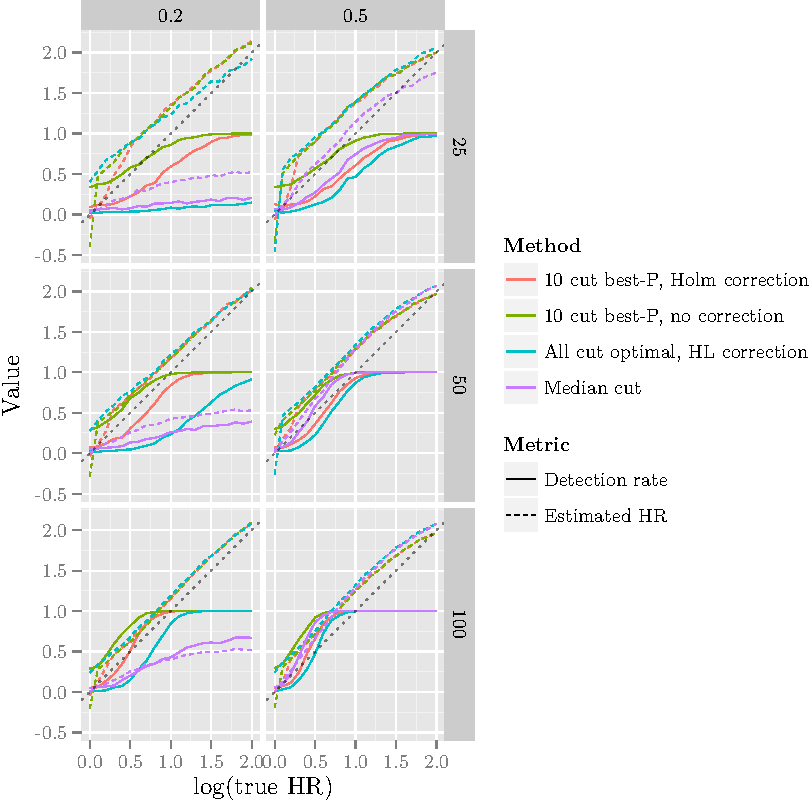
\includegraphics[width=\maxwidth]{figure/02-exp1-plots-1} 

}


\begin{kframe}\begin{alltt}
\hlkwd{ggplot}\hlstd{(exp1.result.melted[exp1.result.melted}\hlopt{$}\hlstd{censoring.rate} \hlopt{==} \hlnum{0.5} \hlopt{& !}\hlstd{(exp1.result.melted}\hlopt{$}\hlstd{Metric} \hlopt \hlkwd{c}\hlstd{(}\hlstr{"failrate"}\hlstd{,} \hlstr{"censrate"}\hlstd{)),],} \hlkwd{aes}\hlstd{(}\hlkwc{x} \hlstd{= log.hazard.ratio,} \hlkwc{y} \hlstd{= value,} \hlkwc{colour} \hlstd{= Method,} \hlkwc{lty} \hlstd{= Metric))} \hlopt{+}
        \hlkwd{geom_line}\hlstd{()} \hlopt{+}
        \hlkwd{facet_grid}\hlstd{(cohort.size} \hlopt{~} \hlstd{class.1.fraction)} \hlopt{+}
        \hlkwd{geom_abline}\hlstd{(}\hlkwc{intercept} \hlstd{=} \hlnum{0}\hlstd{,} \hlkwc{slope} \hlstd{=} \hlnum{1}\hlstd{,} \hlkwc{alpha} \hlstd{=} \hlnum{0.5}\hlstd{,} \hlkwc{linetype} \hlstd{=} \hlstr{"dotted"}\hlstd{)} \hlopt{+}
        \hlkwd{coord_fixed}\hlstd{()} \hlopt{+}
        \hlkwd{labs}\hlstd{(}\hlkwc{x} \hlstd{=} \hlstr{"log(true HR)"}\hlstd{,} \hlkwc{y} \hlstd{=} \hlstr{"Value"}\hlstd{)}
\end{alltt}
\end{kframe}

{\centering 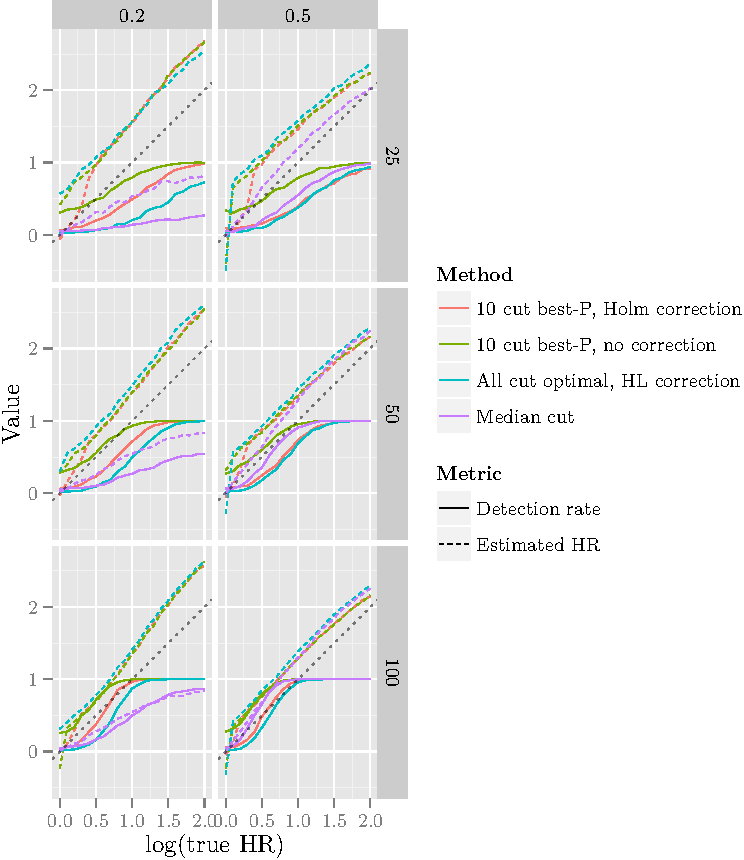
\includegraphics[width=\maxwidth]{figure/02-exp1-plots-2} 

}


\begin{kframe}\begin{alltt}
\hlkwd{ggplot}\hlstd{(exp1.result.melted[exp1.result.melted}\hlopt{$}\hlstd{censoring.rate} \hlopt{==} \hlnum{0.2} \hlopt{&} \hlstd{exp1.result.melted}\hlopt{$}\hlstd{Metric} \hlopt{==} \hlstr{"Detection rate"}\hlstd{,],} \hlkwd{aes}\hlstd{(}\hlkwc{x} \hlstd{= log.hazard.ratio,} \hlkwc{y} \hlstd{= value,} \hlkwc{colour} \hlstd{= Method))} \hlopt{+}
        \hlkwd{geom_line}\hlstd{()} \hlopt{+}
        \hlkwd{facet_grid}\hlstd{(class.1.fraction} \hlopt{~} \hlstd{cohort.size)} \hlopt{+}
        \hlkwd{labs}\hlstd{(}\hlkwc{x} \hlstd{=} \hlstr{"log(true HR)"}\hlstd{,} \hlkwc{y} \hlstd{=} \hlstr{"Detection rate"}\hlstd{)} \hlopt{+}
        \hlkwd{theme_bw}\hlstd{()} \hlopt{+} \hlkwd{theme}\hlstd{(}\hlkwc{legend.position} \hlstd{=} \hlstr{"bottom"}\hlstd{)}
\end{alltt}
\end{kframe}

{\centering 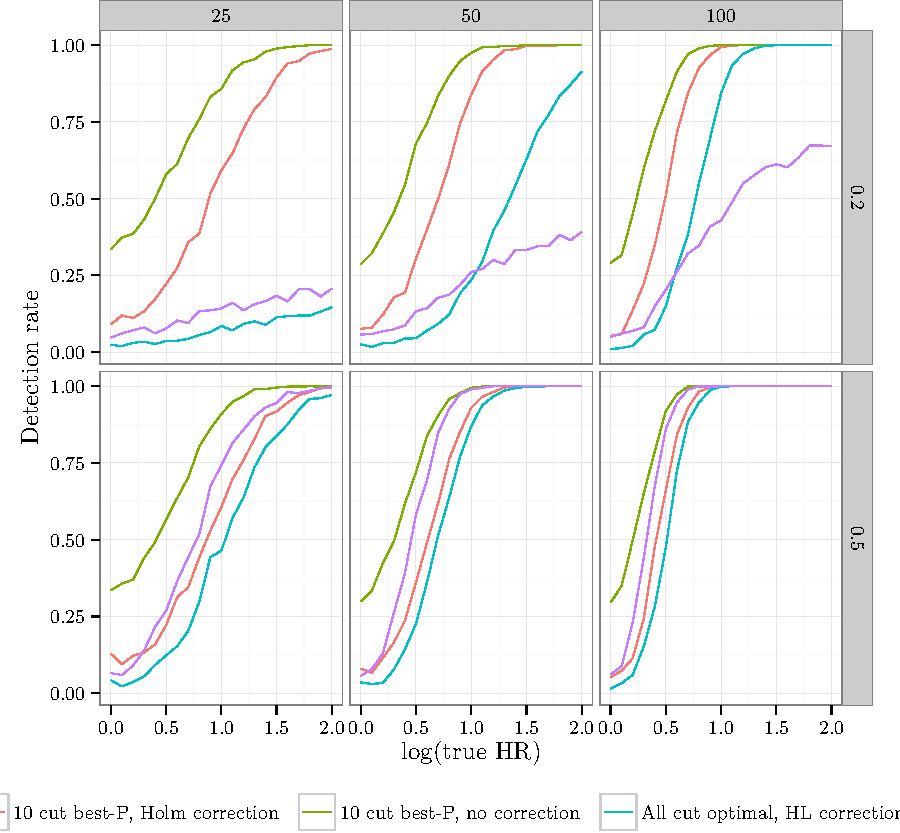
\includegraphics[width=\maxwidth]{figure/02-exp1-plots-3} 

}


\begin{kframe}\begin{alltt}
\hlkwd{ggplot}\hlstd{(exp1.result.melted[exp1.result.melted}\hlopt{$}\hlstd{censoring.rate} \hlopt{==} \hlnum{0.5} \hlopt{&} \hlstd{exp1.result.melted}\hlopt{$}\hlstd{Metric} \hlopt{==} \hlstr{"Detection rate"}\hlstd{,],} \hlkwd{aes}\hlstd{(}\hlkwc{x} \hlstd{= log.hazard.ratio,} \hlkwc{y} \hlstd{= value,} \hlkwc{colour} \hlstd{= Method))} \hlopt{+}
        \hlkwd{geom_line}\hlstd{()} \hlopt{+}
        \hlkwd{facet_grid}\hlstd{(class.1.fraction} \hlopt{~} \hlstd{cohort.size)} \hlopt{+}
        \hlkwd{labs}\hlstd{(}\hlkwc{x} \hlstd{=} \hlstr{"log(true HR)"}\hlstd{,} \hlkwc{y} \hlstd{=} \hlstr{"Detection rate"}\hlstd{)} \hlopt{+}
        \hlkwd{theme_bw}\hlstd{()} \hlopt{+} \hlkwd{theme}\hlstd{(}\hlkwc{legend.position} \hlstd{=} \hlstr{"bottom"}\hlstd{)}
\end{alltt}
\end{kframe}

{\centering 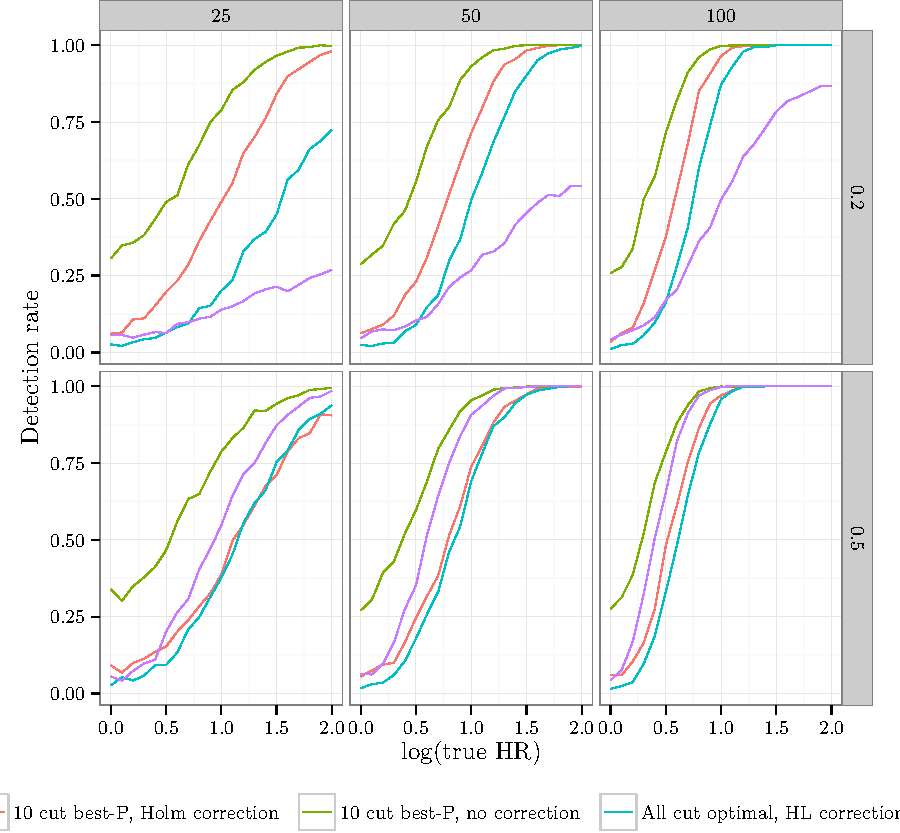
\includegraphics[width=\maxwidth]{figure/02-exp1-plots-4} 

}


\begin{kframe}\begin{alltt}
\hlkwd{ggplot}\hlstd{(exp1.result.melted[exp1.result.melted}\hlopt{$}\hlstd{censoring.rate} \hlopt{==} \hlnum{0.2} \hlopt{&} \hlstd{exp1.result.melted}\hlopt{$}\hlstd{Metric} \hlopt{==} \hlstr{"Estimated HR"}\hlstd{,],} \hlkwd{aes}\hlstd{(}\hlkwc{x} \hlstd{= log.hazard.ratio,} \hlkwc{y} \hlstd{= value,} \hlkwc{colour} \hlstd{= Method))} \hlopt{+}
        \hlkwd{geom_line}\hlstd{()} \hlopt{+}
        \hlkwd{facet_grid}\hlstd{(class.1.fraction} \hlopt{~} \hlstd{cohort.size)} \hlopt{+}
        \hlkwd{geom_abline}\hlstd{(}\hlkwc{intercept} \hlstd{=} \hlnum{0}\hlstd{,} \hlkwc{slope} \hlstd{=} \hlnum{1}\hlstd{,} \hlkwc{alpha} \hlstd{=} \hlnum{0.5}\hlstd{)} \hlopt{+}
        \hlkwd{coord_fixed}\hlstd{()} \hlopt{+}
        \hlkwd{labs}\hlstd{(}\hlkwc{x} \hlstd{=} \hlstr{"log(true HR)"}\hlstd{,} \hlkwc{y} \hlstd{=} \hlstr{"log(estimated HR)"}\hlstd{)} \hlopt{+}
        \hlkwd{theme_bw}\hlstd{()} \hlopt{+} \hlkwd{theme}\hlstd{(}\hlkwc{legend.position} \hlstd{=} \hlstr{"bottom"}\hlstd{)}
\end{alltt}
\end{kframe}

{\centering 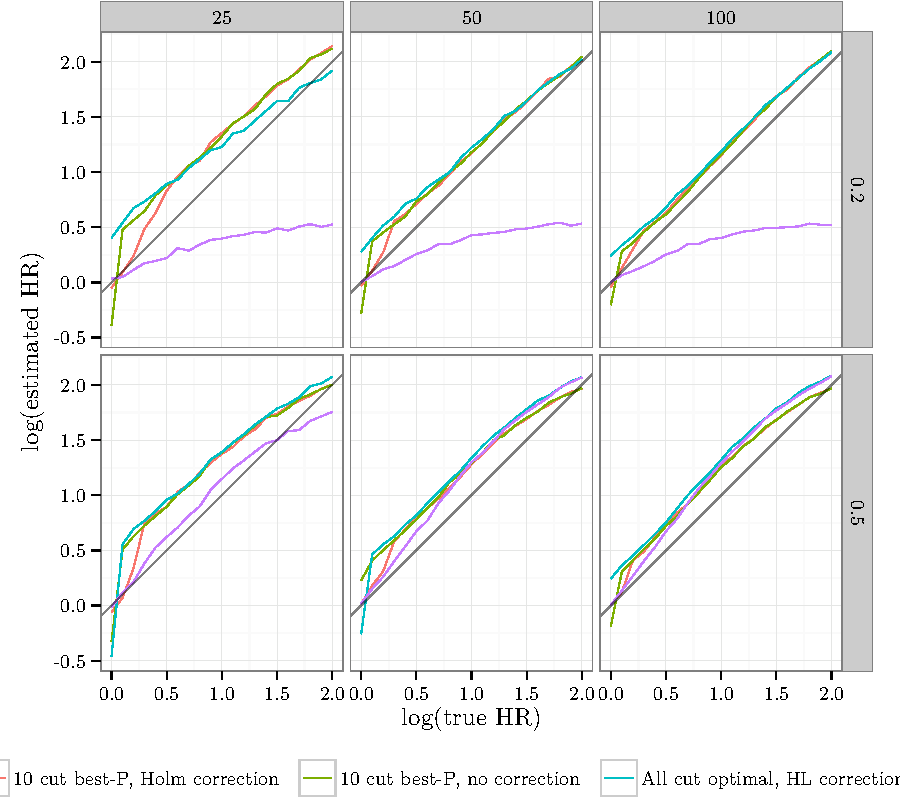
\includegraphics[width=\maxwidth]{figure/02-exp1-plots-5} 

}


\begin{kframe}\begin{alltt}
\hlkwd{ggplot}\hlstd{(exp1.result.melted[exp1.result.melted}\hlopt{$}\hlstd{censoring.rate} \hlopt{==} \hlnum{0.5} \hlopt{&} \hlstd{exp1.result.melted}\hlopt{$}\hlstd{Metric} \hlopt{==} \hlstr{"Estimated HR"}\hlstd{,],} \hlkwd{aes}\hlstd{(}\hlkwc{x} \hlstd{= log.hazard.ratio,} \hlkwc{y} \hlstd{= value,} \hlkwc{colour} \hlstd{= Method))} \hlopt{+}
        \hlkwd{geom_line}\hlstd{()} \hlopt{+}
        \hlkwd{facet_grid}\hlstd{(class.1.fraction} \hlopt{~} \hlstd{cohort.size)} \hlopt{+}
        \hlkwd{geom_abline}\hlstd{(}\hlkwc{intercept} \hlstd{=} \hlnum{0}\hlstd{,} \hlkwc{slope} \hlstd{=} \hlnum{1}\hlstd{,} \hlkwc{alpha} \hlstd{=} \hlnum{0.5}\hlstd{)} \hlopt{+}
        \hlkwd{coord_fixed}\hlstd{()} \hlopt{+}
        \hlkwd{labs}\hlstd{(}\hlkwc{x} \hlstd{=} \hlstr{"log(true HR)"}\hlstd{,} \hlkwc{y} \hlstd{=} \hlstr{"log(estimated HR)"}\hlstd{)} \hlopt{+}
        \hlkwd{theme_bw}\hlstd{()} \hlopt{+} \hlkwd{theme}\hlstd{(}\hlkwc{legend.position} \hlstd{=} \hlstr{"bottom"}\hlstd{)}
\end{alltt}
\end{kframe}

{\centering 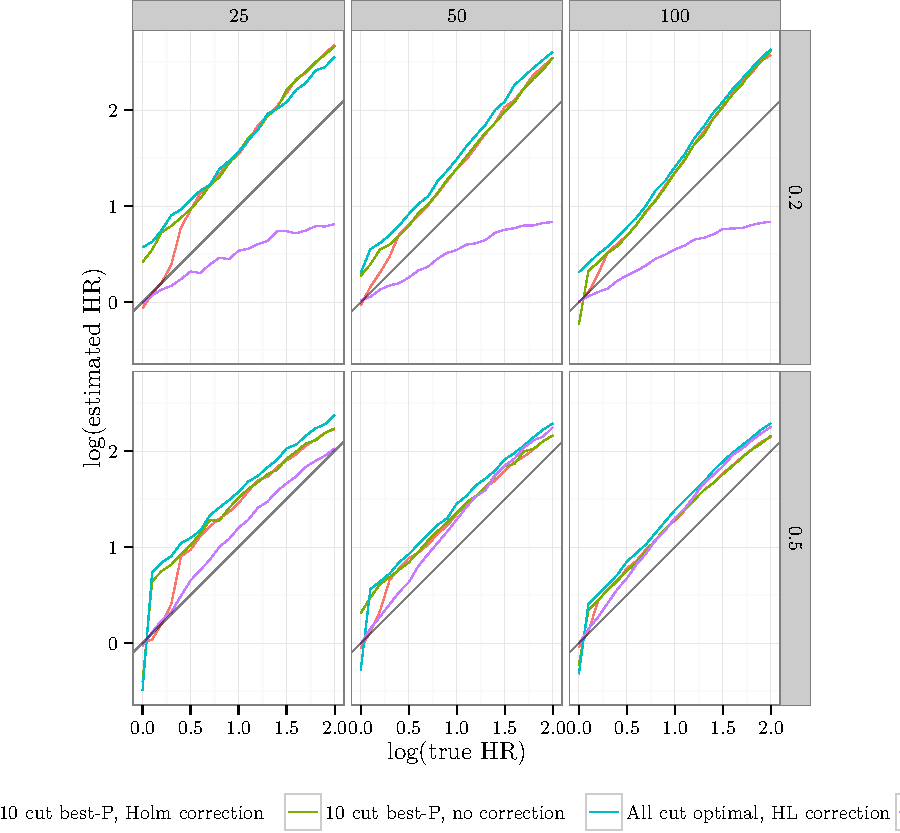
\includegraphics[width=\maxwidth]{figure/02-exp1-plots-6} 

}



\end{knitrout}

\end{document}
